\documentclass[12pt]{article}
\usepackage[utf8]{inputenc}
\usepackage{multirow}
\usepackage{float}
\usepackage{indentfirst}
\usepackage{graphicx}
\usepackage[document]{ragged2e}
\usepackage{pdfpages}
\usepackage{subcaption}
\usepackage[a4paper, total={7in, 10.6in}]{geometry}
\usepackage{times}
\renewcommand{\contentsname}{İçindekiler}
\renewcommand{\figurename}{Şekil}

%%%%%%%%%%%%%%%%%%%%%%%%%%%%%%%%%%%%%%%%%%%%%%%%%%%%
%          3. Tekil Şahıs Kullanılacaktır          %
%   Figürlerin caption'u altta, Tabloların üstte   %
%%%%%%%%%%%%%%%%%%%%%%%%%%%%%%%%%%%%%%%%%%%%%%%%%%%%


\title{BLM3022\\
Ağ Teknolojileri\\
Proje Raporu\\
Proje İsmi: Sunucu Tarafı Otomatik Servis Keşfi}
\date{2021-2022 Bahar Dönemi}


\begin{document}
\maketitle
\begin{justify}

% Please add the following required packages to your document preamble:
% \usepackage{multirow}
\begin{table}[H]
\centering
\label{tab:my-table}
\begin{tabular}{|c|c|c|l|}
\hline
\textbf{Grup Sorumlusu}    & Metin Usta      & \%25 & Sistem tasarımı ve Sistemin test edilmesi\\ \hline
\multirow{3}{*}{} & İsmet Güngör    & \%25 & Sistem tasarımı ve Servislerin gerçeklenmesi\\ \cline{2-4} 
                  & Emre Arslanoğlu & \%25 & Sistem hakkında ön bilgi toplanması \\ \cline{2-4} 
                  & Umutcan Sevdi   & \%25 & Sistem tasarımı ve Sistemin gerçeklenmesi \\ \hline
\end{tabular}
\end{table}

\tableofcontents
\pagebreak

% - Metin
%%%%%%%%%%%%%%%%%%%%%%%%%%%%%%%%%%%%%%%%%%%%
\section{Proje Tanımı}
Herhangi bir alanda bir hizmet veren sistemler, ilk kurulduklarında küçük boyutlu başlayabilseler de zaman içinde birçok değişime ve genişlemeye maruz kalırlar. Hatta bazen bu değişiklikler ve genişlemeler, sistemin yaşam döngüsü boyunca devam eder. Bu tür durumlarda sistemden hizmet almak için sürekli olarak yeni bir yol kullanmak gerekebilir.

Sistemlerin yaşadığı değişimlerin ve genişlemelerin, o sistemden hizmet alınmasının önüne geçmemesi için ek araçlara ve yapılara ihtiyaç duyulur. Bu yapıya “Servis Keşfi” adı verilir. Eğer bu yapının gerçekleştirdiği işlevler tamamen sunucu tarafında yapılarak kullanıcının yükü hafifletiliyorsa buna “Sunucu Tarafı Servis Keşfi” denir.

Şekil \ref{fig:disc}’de kullanıcı, servis keşfi yapısı ve servis hizmeti sağlayan sunucular ve aradaki ilişkiler gösterilmiştir.

\begin{figure}[H]
    \centering
    \includegraphics[width=0.7\linewidth]{pdfs/ServerSideDiscovery.pdf}
    \caption{Sunucu Tarafı Servis Keşfi}
    \label{fig:disc}
\end{figure}

Proje kapsamında Servis Defteri(Service Registry) yapısı ile Yük Dağıtıcısı(Load Balancer) birleştirilecek ve var olan servis sağlayıcıları veritabanı benzeri bir sistemde kaydedilmek yerine UDP ile yapılacak olan yayın(broadcast) sonucu bulunacaktır.
Şekil \ref{fig:autodisc}'de projede gerçeklenecek olan sistemin yapısı verilmiştir.

\begin{figure}[H]
    \centering
    \includegraphics[width=0.7\linewidth]{pdfs/ServerSideAutoDiscovery.pdf}
    \caption{Sunucu Tarafı Otomatik Servis Keşfi}
    \label{fig:autodisc}
\end{figure}

\subsection{Ön İnceleme}
Bu bölümde, sunucu tarafı servis keşfinde kullanılan uygulamalar ve mimarileri incelenmiştir.

\textbf{Consul}

Consul, servis ağlarının yönetimi, keşfi, konfigüre edilmesi, güvenliğinin sağlanması ve sağlık durumlarının kontrol edilmesi gibi birçok görevi yerine getirir.

Consul mimarisinin servis keşfi ve servislerin konfigüre edilmesi ile alakalı kısımları Şekil \ref{fig:consul}'de verilmiştir.

\begin{figure}[H]
    \centering
    \includegraphics[width=0.7\linewidth]{pdfs/ConsulArchitecture.pdf}
    \caption{Consul Mimarisi}
    \label{fig:consul}
\end{figure}

Bu mimaride Kayıt Defteri yapısı proje kapsamında gerçekleştirilecek olan mimari ile benzer olarak aynı zamanda yük dengeleme işleminden de sorumludur.

Consul dışında servis keşfi ve daha birçok işlevin yerine getirilmesini sağlayan araçlara örnek olarak:

\begin{itemize}
    \item Apache Zookeeper
    \item Etcd
    \item Eureka
\end{itemize}
verilebilir.

\subsection{Artılar}
Bu kısımda geliştirilecek olan sistemin diğer sistemlere ve geleneksel servis keşfi metotlarına göre artıları incelenmiştir.

\begin{enumerate}
    \item Var olan servisleri UDP kullanarak keşfettiği için dinamik değişimlerden etkilenmez.
    \item Yük dengeleyici ve servis defteri aynı yapı içerisinde bulunduğu için kullanıcının servise erişimini dolaysız bir şekilde gerçekleştirmesini sağlar.
    \item Keşfedilen servislerden sağlık değeri yüksek olan ile kullanıcı tarafı bağlantı kuracağı için sunucu üzerindeki yük kaldırılmış olur.
\end{enumerate}

\subsection{Eksiler}
Bu kısımda geliştirilecek olan sistemin diğer sistemlere ve geleneksel servis keşfi metotlarına göre eksileri incelenmiştir.

\begin{enumerate}
    \item Birçok yapının tek bir yapı altında birleştirilmesinden dolayı single-point of failure probleminin getirdiği sorunlardan etkilenir.
    \item Adresleri yüksek bitlerde birbirinden farklı olan ve aynı alt ağ içerisinde toplanamayan servis sayısı arttıkça yayın yapılacak noktaların kaydedilmesi gerekir.
\end{enumerate}
%%%%%%%%%%%%%%%%%%%%%%%%%%%%%%%%%%%%%%%%%%%%

% - İsmet
%%%%%%%%%%%%%%%%%%%%%%%%%%%%%%%%%%%%%%%%%%%%
\section{Sistem Mimarisi}

Sistem 3 farklı aktörün ortak çalışması ile sağlanmaktadır. Bu aktörler:
\begin{itemize}
    \item Kullanıcı
    \item Sunucu
    \item Servis
\end{itemize}
Bu aktörlerin iletişimi; kullanıcı-servis arasında TCP ile, servis-sunucu arasında UDP ile ve kullanıcı-sunucu arasında da TCP ile sağlanmaktadır. Kullanıcının sunucu tarafından belirlenmiş ve sistem içerisinde bulunan servislerden seçim yaparak bunu sunucuya iletmesi ile başlamaktadır. Sunucu tarafından UDP ile broadcast metodunda istenilen hizmet servislere iletilecek ve uygun olan servisler tarafından yoğunlukları ile birlikte geri dönüş yapılacaktır. Bu sayede sunucu kullanıcı tarafından istenilen servise uygun sunucuyu seçerken, sunucuların yoğunluklarını da inceleyerek sunucuları overwhelm etmeden "servis keşfi" ve "yük dengeleme" sağlanacaktır. Sunucu tarafından uygun bulunan servisin bağlantı için gerekli bilgileri kullanıcı ile paylaşılmaktadır. Kullanıcı, sunucudan aldığı bilgiler ile servise istek atarak TCP protokolünde bağlantı kuracak ve talep ettiği hizmetten yararlanmaktadır. İletişim şeması Şekil \ref{fig:system_diagram}'te gösterilmiştir.

\begin{figure}[H]
    \centering
    \includegraphics[width=1\linewidth]{pdfs/sistem_sema.pdf}
    \caption{Sistem Şeması}
    \label{fig:system_diagram}
\end{figure}

\subsection{Kullanıcı}
Kullanıcı, sistem içerisinde hizmet almak için bulunmaktadır. Kullanıcı TCP bağlantı ilkelerini sağlayabilen herhangi bir cihaz olabilir. Kullanıcının sistemde görevi Sunucu ile TCP protokolü ile iletişim kurarak, sunucuda izin verilen hizmetler birini istemek ve dönüt beklemektir. Dönüt olarak sunucudan "en uygun" servisle iletişim kurması için gerekli bilgiler dönmektedir. Bu sayede uygun servisin bulunması için fazladan efor harcamadan istediği hizmete uygun servise ulaşabilmektedir. Sunucu tarafından servislerin sahip olduğu yük değerlendirildiği için en uygun servisten hizmet alarak trafikte zaman kaybetmeden istediği hizmete erişebilmektedir.

\begin{enumerate}
    \item[--]Kullanıcı-Sunucu iletişiminde TCP protokolünün seçilme sebepleri:
    \begin{itemize}
        \item Kullanıcının sadece TCP protokolü ile sunucu üzerinden iletişim kurması sayesinde sunucu ile olan iletişim güvenilir şekilde sağlanmaktadır ve hatalara karşı daha duyarlıdır.
        \item Kullanıcı-Sunucu iletişiminde veri aktarım düzeyi sınırlı bir seviyede olduğu için UDP protokolünün sunduğu hızın aksine TCP protokolünün sunduğu güvenilirlik tercih edilmiştir.
    \end{itemize}
    \item[--] Kullanıcı-Servis iletişiminde TCP protokolünün seçilme sebepleri:
    \begin{itemize}
        \item Servis ile bağlantının TCP protokolü ile gerçekleştirilmesi sayesinde uygulama katmanında ekstra eklentilere gerek kalmadan güvenilir iletişim kurulmaktadır. 
        \item Aktarılan veri miktarının fazla olmasına rağmen kurulacak olan uçtan-uca iletşimin karşılıklı veri aktarımı sağlaması sebebiyle TCP protokolü tercih edilmiştir.
    \end{itemize}
\end{enumerate}

\subsection{Sunucu}
Sunucu, sistem içerisinde hizmet almak isteyen kullanıcıya en uygun servisin bağlantı için gerekli bilgilerini iletmek için bulunmaktadır. Sunucu, sistemden hizmet almak isteyen kullanıcı ile bağlantı kurar ve sistem içerisinde erişilebilir olan hizmetlerden seçilmiş olan hizmetin bilgisini alır. Bu hizmete uygun servisleri bulmak adına UDP protokolünde broadcast yayın yapar. Hizmeti sağlayabilecek olan servisler tarafından sunucuya yük bilgileri iletilir. Sunucu gelen yük bilgilerini karşılaştırarak en uygun servisi seçer. Seçilen servisin iletişim için gerekli olan bilgileri hizmet almak isteyen kullanıcıya iletilir.
\begin{enumerate}
    \item[--] Sunucu-Kullanıcı iletişiminde TCP protokolünün seçilme sebepleri:
    \begin{itemize}
        \item Sunucu ile iletişime geçen kullanıcın takibinin yapılmasını sağlamaktadır.
        \item TCP bağlantısının kopma süresi tamamlanmadan bağlantıya dönüş yapılarak ek bağlantılara ve yeni iletişim başlatmaya gerek kalmadan veri aktarımını sağlamak adına tercih edilmiştir.
    \end{itemize}
    \item[--] Sunucu-Servis iletişiminde UDP protokolünün seçilme sebepleri:
    \begin{itemize}
        \item Sisteme servislerin dinamik bir şekilde eklenebilmesi ve erişim için ek bağlantılar kurulmaması için broadcast yayın tercih edilmiştir.
        \item  Broadcast yayın yapılabilmesi için UDP protokolünün tercih edilmesi gerekmektedir.
    \end{itemize}
\end{enumerate}


\subsection{Servis}
Servis, hizmet almak isteyen kullanıcıya hizmet vermek için bulunmaktadır. Servis, sunucu tarafından yapılan UDP protokolündeki broadcast yayındaki istenen hizmetin bilgisini alır. Alınan veri incelenir eğer servisin sağlayabildiği bir hizmet ise sunucu ile TCP protokolünde bağlantı kurularak servisin sahip olduğu yük bilgisi sunucuya gönderilir.
\begin{enumerate}
    \item[--] Servis-Kullanıcı iletişiminde TCP protokolünün seçilme sebepleri:
    \begin{itemize}
        \item Kullanıcıdan alınacak olan verinin güvenilirliği için TCP protokolü tercih edilmiştir.
        \item Kullanıcıya verilecek olan hizmetin doğruluğu önemli olduğu için daha güvenilir iletişime sahip olan TCP protokolü tercih edilmiştir.
    \end{itemize}
    \item[--] Servis-Sunucu iletişiminde TCP protokolünün seçilme sebepleri:
    \begin{itemize}
        \item UDP protokolü ile yapılan broadcast yayınına servisin sahip olduğu yükün ve IP adresinin sunucuya iletiminin güvenilir şekilde gerçekleştirilmesi için tercih edilmiştir.
        \item Sunucuya birden fazla servisin cevap verdiği durumda gelen cevapların karışmaması ve servis sağlayıcılarının karışmaması için tercih edilmiştir.
    \end{itemize}
\end{enumerate}


%%%%%%%%%%%%%%%%%%%%%%%%%%%%%%%%%%%%%%%%%%%%
\section{Uygulama}
%%%%%%%%%%%%%%%%%%%%%%%%%%%%%%%%%%%%%%%%%%%%
Bu bölümde tasarlanan sistem \textbf{Java} dili ile kodlanarak çalışmaya hazır hale getirilmiştir. Yapı test edilmek için halinde saat bilgisi, verilen adresin dns bilgisini döndürme gibi servisler prototip halde kodlanmıştır. Servis çalıştırılmaya başladıktan sonra farklı işletim sistemi ve bilgisayarda da test edilmiştir. Ayrıca servis ve sunucu iki farklı cihazda da çalışabilmektedir.

\begin{figure}[H]
    \centering
    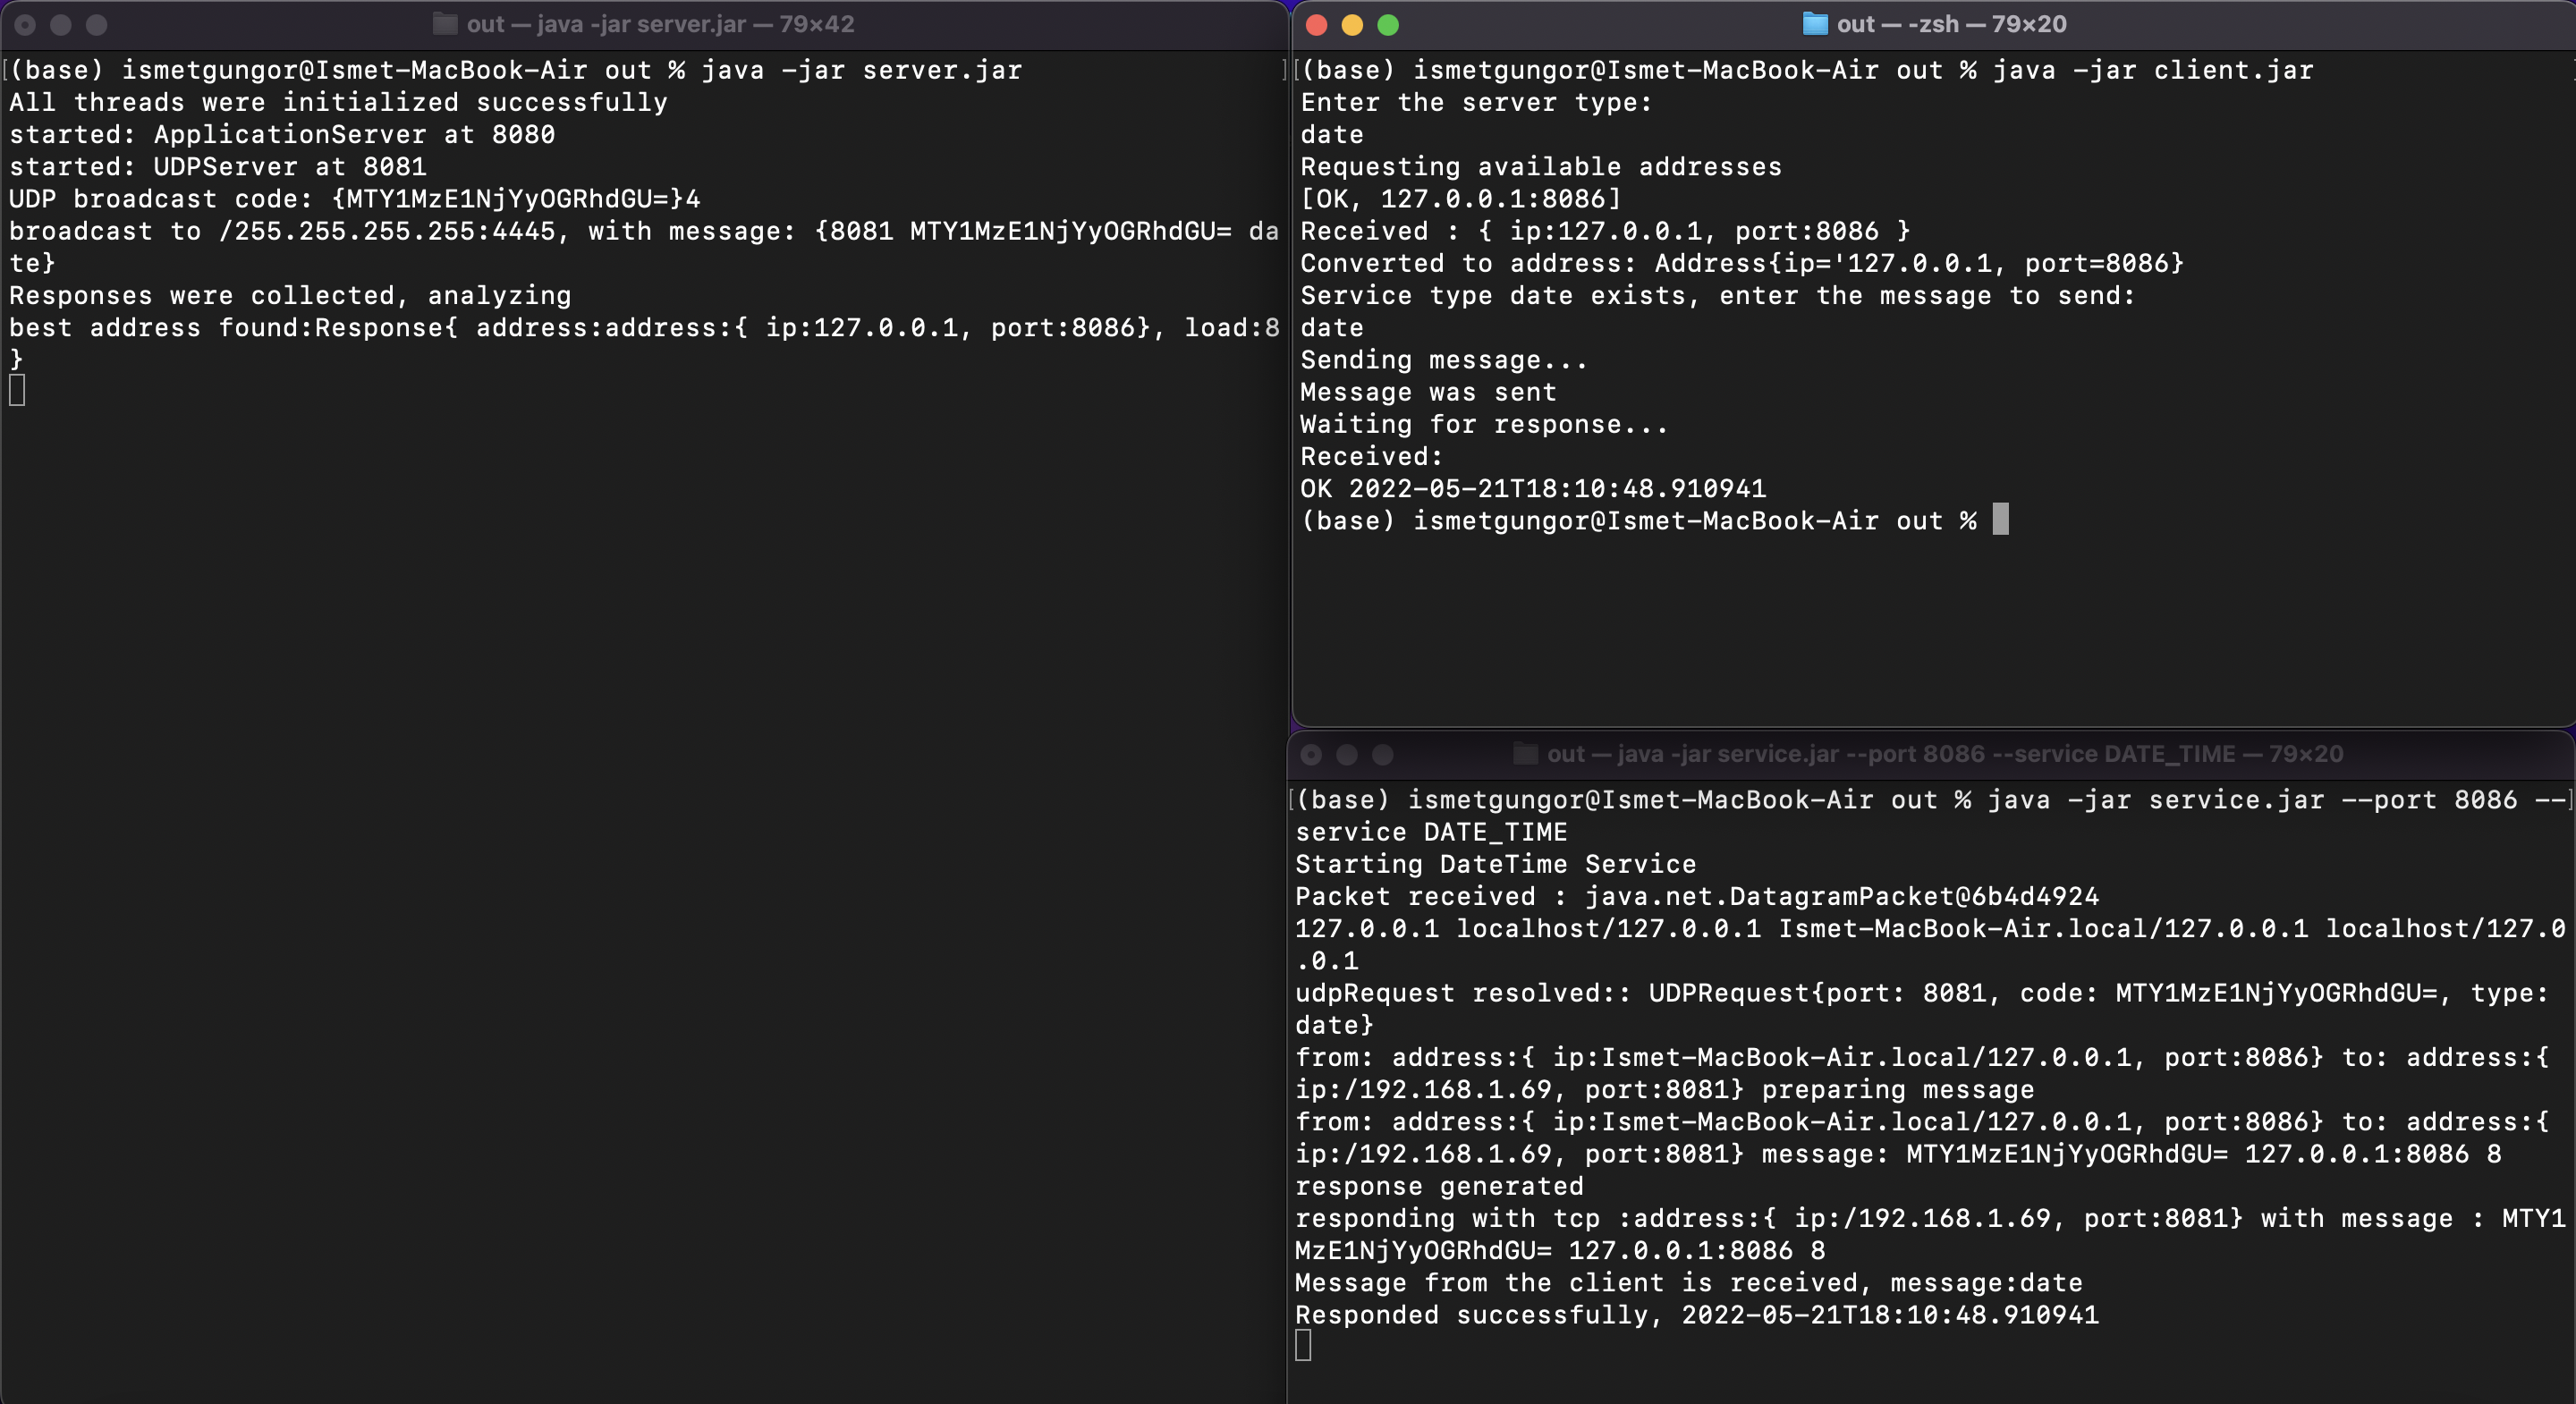
\includegraphics[width=1\linewidth]{pdfs/datetime.png}
    \caption{MacOS işletim sisteminde saat servisi}
    \label{fig:date_time}
\end{figure}

\begin{figure}[H]
    \centering
    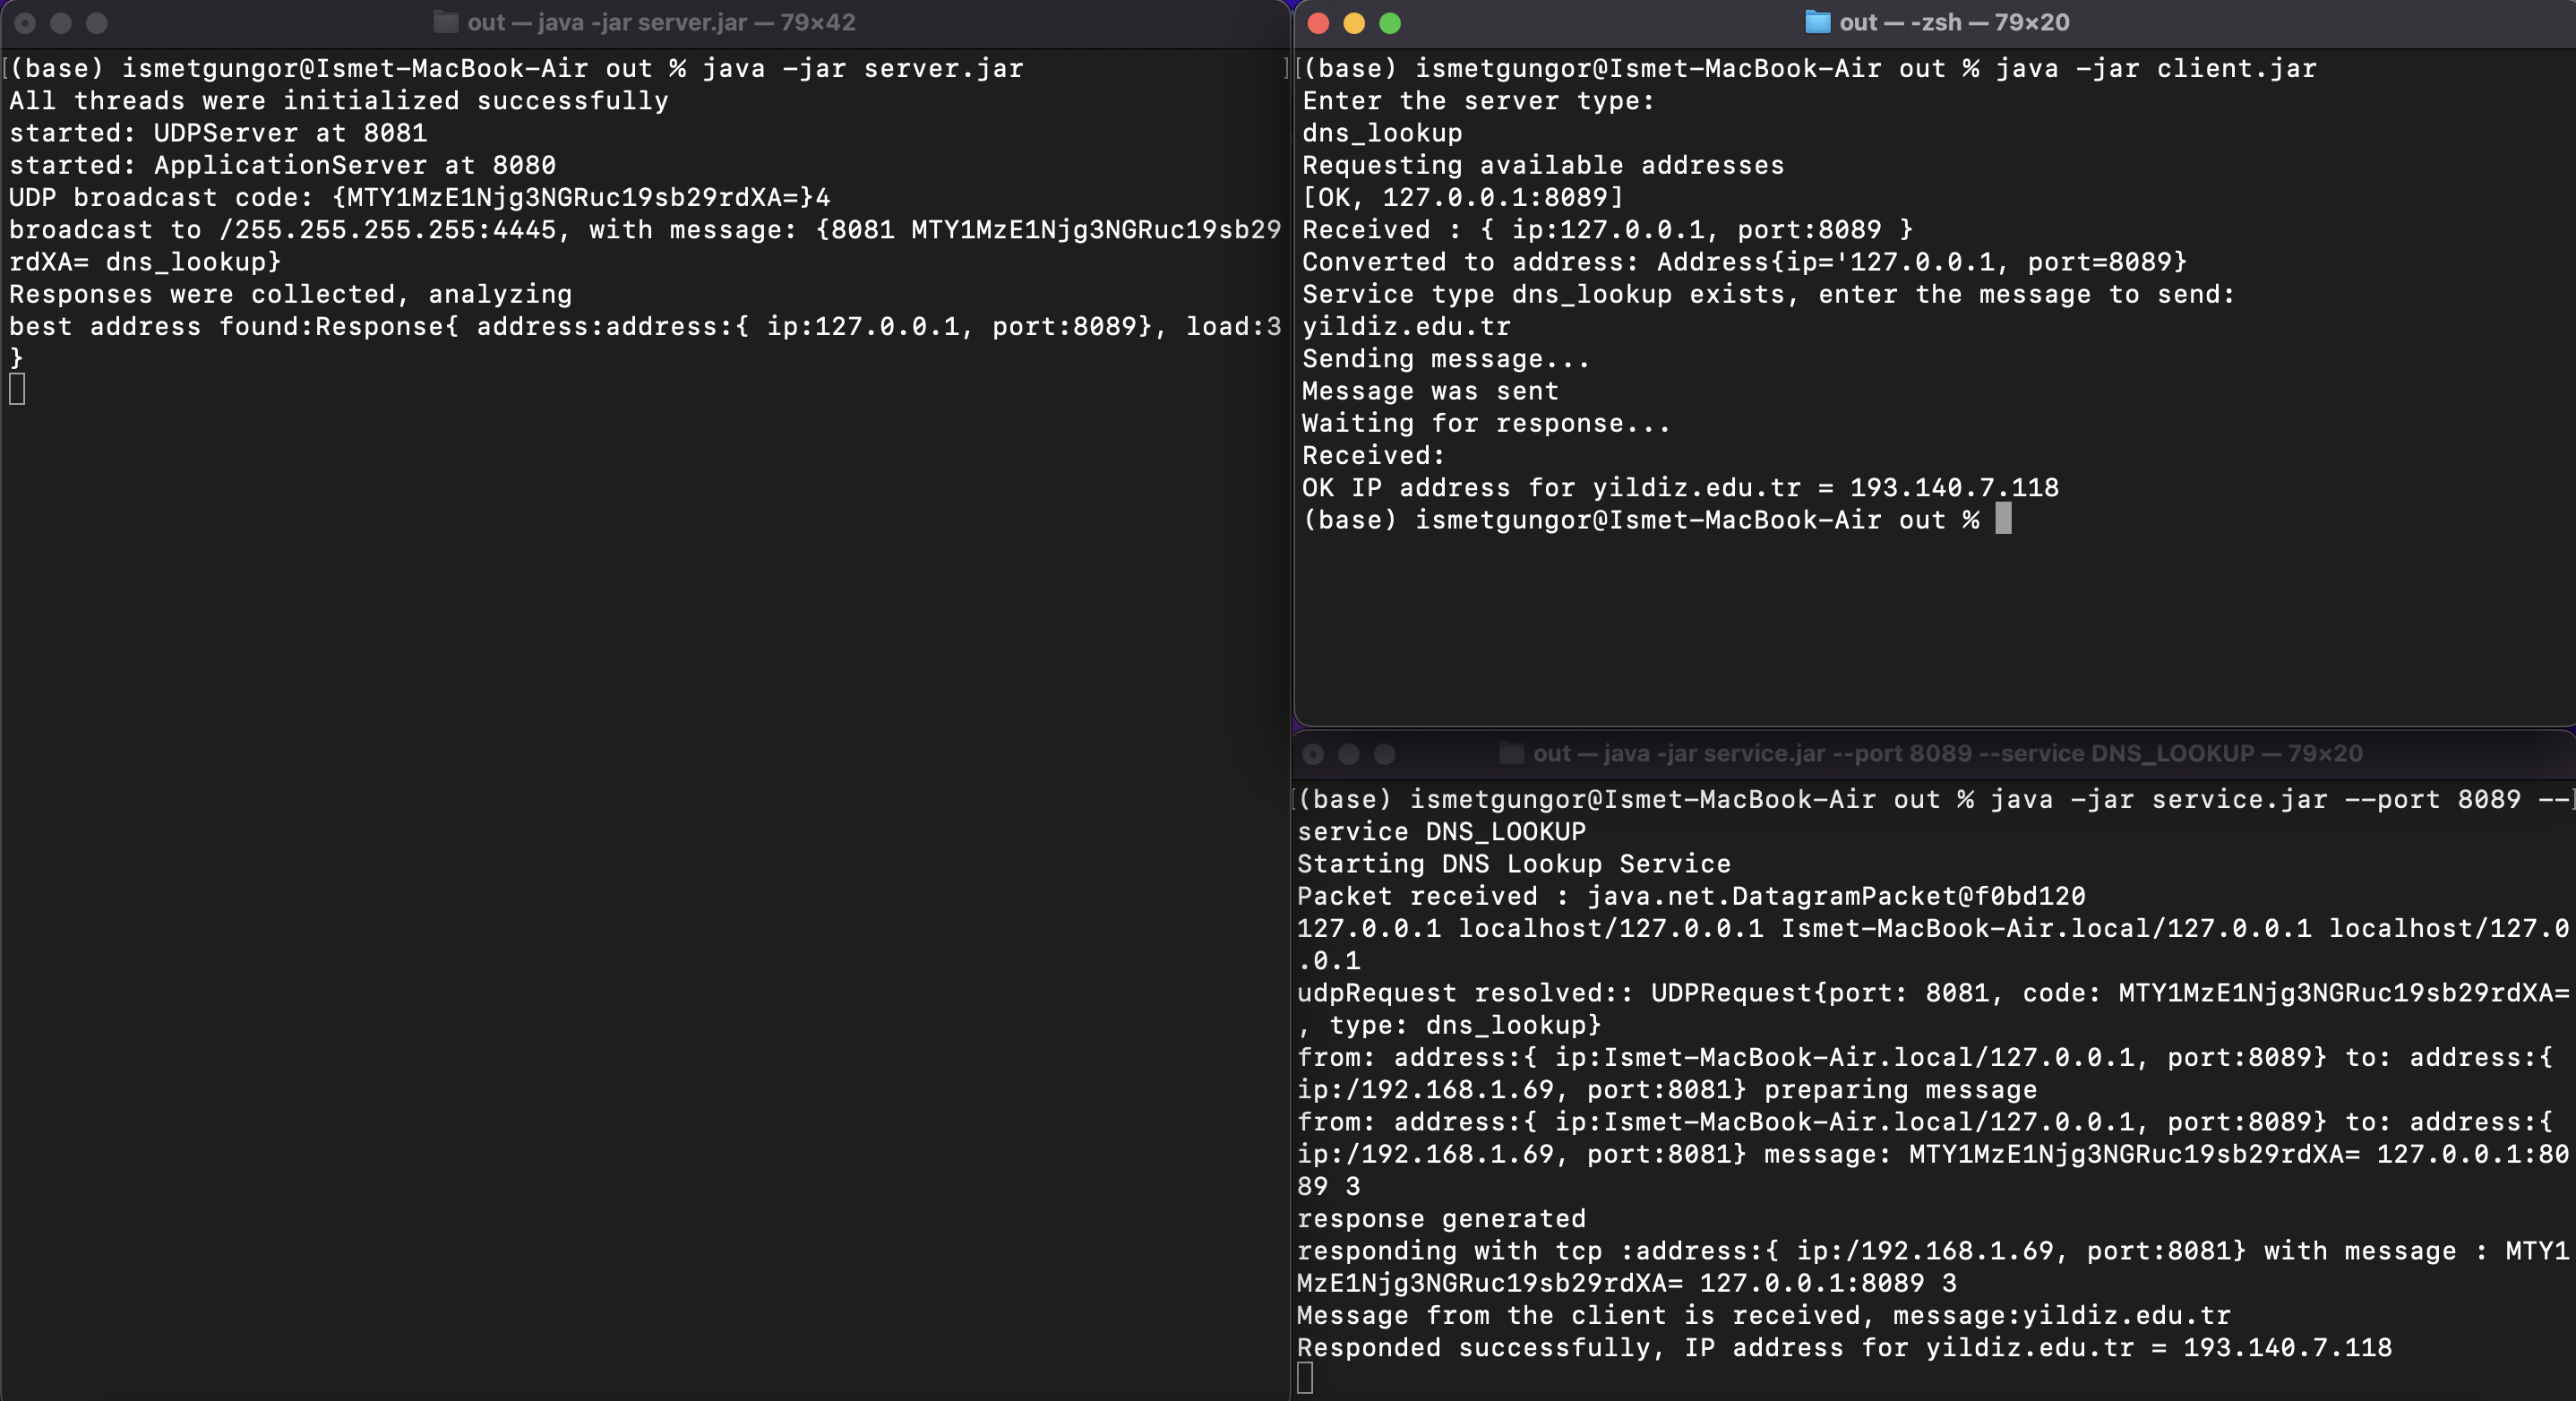
\includegraphics[width=1\linewidth]{pdfs/macdns.png}
    \caption{MacOS işletim sisteminde DNS servisi}
    \label{fig:mac_dns_lookup}
\end{figure}

\begin{figure}[H]
    \centering
    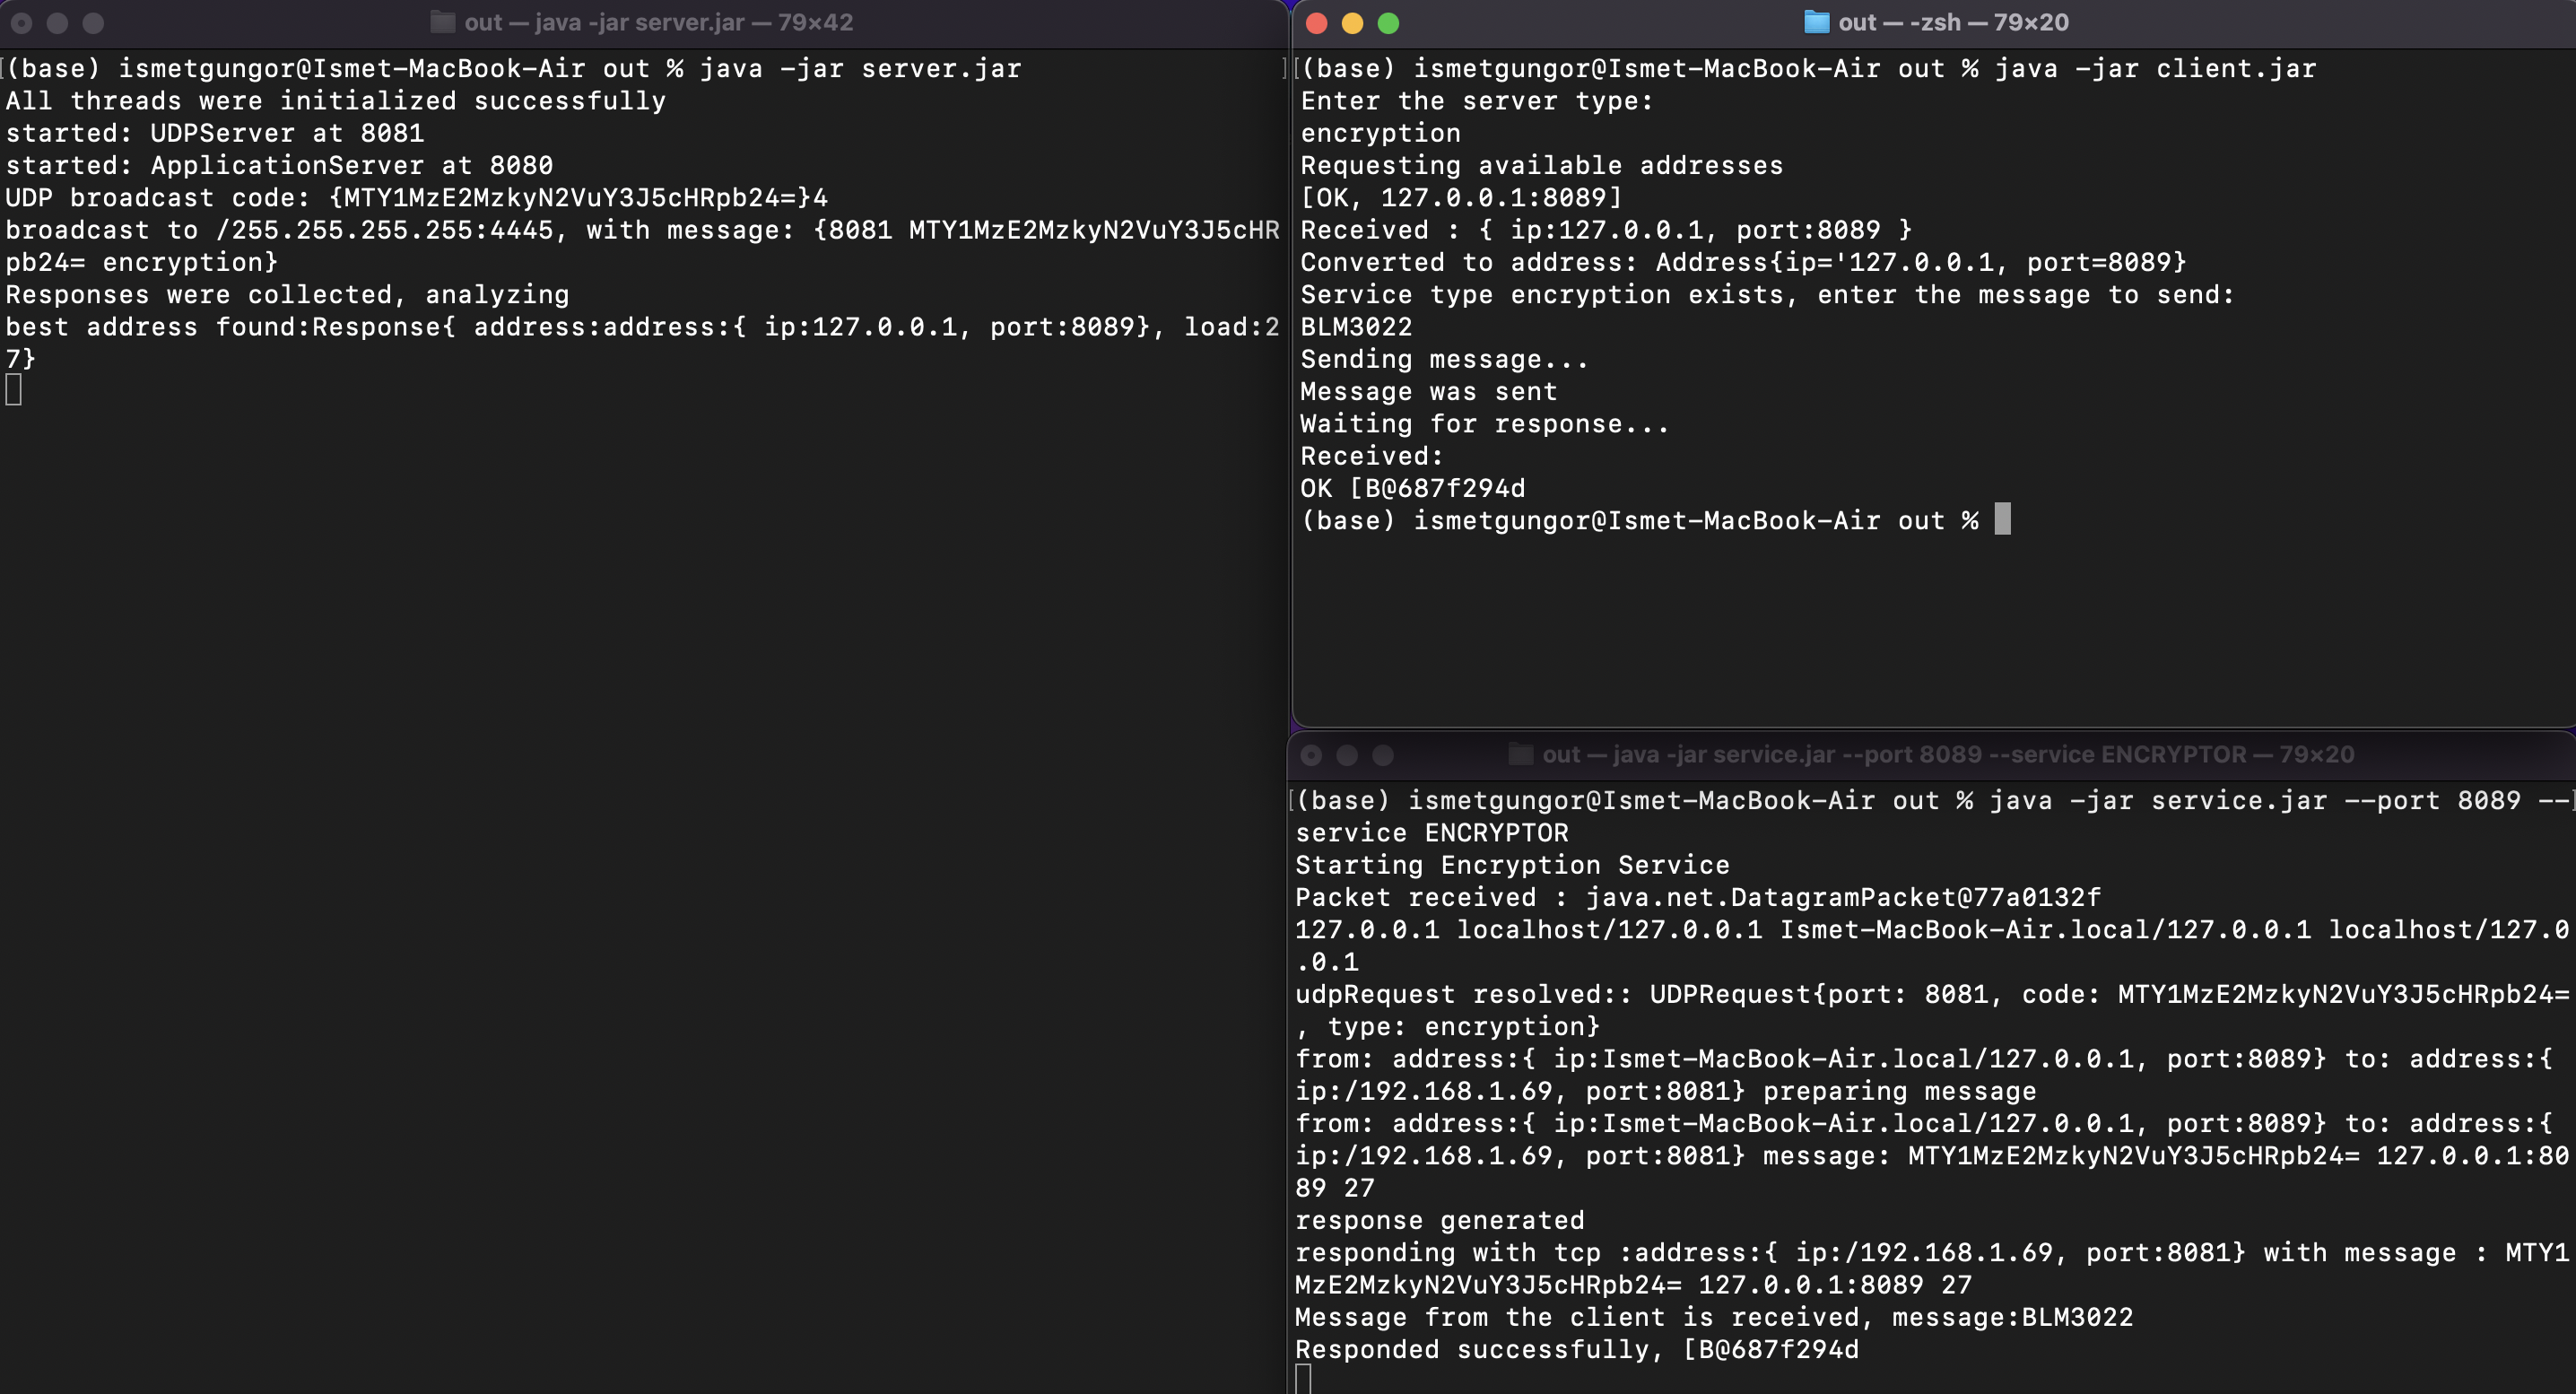
\includegraphics[width=1\linewidth]{pdfs/macosEncryption.png}
    \caption{MacOS işletim sisteminde Encryption servisi}
    \label{fig:mac_encryption}
\end{figure}

% - Emre
%%%%%%%%%%%%%%%%%%%%%%%%%%%%%%%%%%%%%%%%%%%%
\section{Performans Analizi}
Bu bölümde tasarlanan ve gerçekleşen sistem performansı değerlendirilmiş, sistemin pozitif ve negatif yönleriyle analiz edilmiştir. Ayrıca negatif sayılabilecek durumlara karşı geliştirilen alternatif yöntemler geliştirilmiştir.\\


Sistemin performansını değerlendirirken sayısal bir metrik belirlemek oldukça güçtür. Bunun sebebi sistem anlık olarak servisleri keşfetmekte ekstra bir işlem gücü harcarken, sunucuları ve bu sunucuların verdiği servisleri belirlemek adına yapılan güncelleme işlemlerinden kurtarılmaktadır. Ayrıca anlık olarak sisteme eklenen, sistemden düşen, bozulan veya ağır yük altına giren sunucuların durumu yük dengeleyici olarak kullanılan sunucu tarafından hızlıca güncellenecektir. Sistemin performansını belirleme için ise bir yük dengeleyici olarak kullanıldığında saniyede verilen hizmet sayısı bir değerlendirme fonksiyonu olarak kullanılabilmektedir.\\

\subsection{Alternatif Senaryolar}
Sistem ilk tasarlandığında yük dağıtıcı olarak belirlenen sunucu uygulama tarafından aldığı veriyi uygun sunucuya ilettikten sonra hizmet sonucunu tekrar yük dağıtıcı üzerinden uygulamaya iletmekteydi.Şekil \ref{fig:old_model}'de sırayla bağlantı adımları gösterilmiştir.

\begin{figure}[H]
    \centering
    \begin{subfigure}[b]{0.475\textwidth}
        \centering
        \includegraphics[width=1\linewidth]{pdfs/udp_connection.pdf}
        \caption{UDP Bağlantısı}
        \label{fig:udp_diagram}
    \end{subfigure}
    \hfill
    \begin{subfigure}[b]{0.475\textwidth}
        \centering
        \includegraphics[width=1\linewidth]{pdfs/tcp_connection.pdf}
        \caption{TCP Bağlantısı}
        \label{fig:tcp_diagram}
    \end{subfigure}
    \vfill
    \centering
    \begin{subfigure}[b]{0.475\textwidth}
        \centering
        \includegraphics[width=1\linewidth]{pdfs/data_transmission.pdf}
        \caption{Servise Sağlayıcıya Veri Aktarımı}
        \label{fig:data_transmission}
    \end{subfigure}
    \hfill
    \begin{subfigure}[b]{0.475\textwidth}
        \centering
        \includegraphics[width=1\linewidth]{pdfs/result.drawio.pdf}
        \caption{Uygulamaya Veri Aktarımı}
        \label{fig:result}
\end{subfigure}
\caption{Yük Dengeliyici Servis Sağlayıcı İletişim Modeli}
\label{fig:old_model}
\end{figure}

Bu tasarım darboğaz, buffer overflow gibi sorunların oluşma olasılığını arttırdığı için İşlem kapasiteni arttırmak ve yük dağıtıcı yükünü azaltmak adına sistem tasarımında iyileştirmeler yapılmıştır. Yük dağıtıcı servis sağlayıcıları bulduktan sonra uygun servis sağlayıcının IP ve port adreslerini uygulamaya iletir. İşlemler sistemin uç noktalarında gerçekleştirilir. Bu sayede sunucu ağır yük altında bırakılmaz. \ref{fig:new_model}'da tasarlanan bu sistem adım adım görülmektedir. \\

\begin{figure}[H]
    \centering
    \begin{subfigure}[b]{0.475\textwidth}
        \centering
        \includegraphics[width=1\linewidth]{pdfs/udp_system.pdf}
        \caption{UDP Broadcast}
        \label{fig:udp_broadcast}
    \end{subfigure}
    \hfill
    \begin{subfigure}[b]{0.475\textwidth}
        \centering
        \includegraphics[width=1\linewidth]{pdfs/tcp_system.pdf}
        \caption{TCP Bağlantısı}
        \label{fig:tcp_broadcast}
    \end{subfigure}
    \vfill
    \centering
    \begin{subfigure}[b]{0.475\textwidth}
        \centering
        \includegraphics[width=1\linewidth]{pdfs/app_conn.pdf}
        \caption{Uygulama ile IP/Port Paylaşımı}
        \label{fig:app_conn}
    \end{subfigure}
    \hfill
    \begin{subfigure}[b]{0.475\textwidth}
        \centering
        \includegraphics[width=1\linewidth]{pdfs/tcp_app.pdf}
        \caption{Uygulama ile Sistem arasında TCP}
        \label{fig:tcp_app}
    \end{subfigure}
       \caption{Uygulama Servis Sağlayıcı İletişim Modeli}
       \label{fig:new_model}
\end{figure}

% - Emre
%%%%%%%%%%%%%%%%%%%%%%%%%%%%%%%%%%%%%%%%%%%%
\section{Sonuç}
Tasarlanan sistem kodlanmış ve test edilmiştir. Gerçeklenen sistem stabil olarak çalışmakla birlikte farklı platformlar üzerinde çalışabilmektedir. Otomatik servis keşfi yöntemi bu rapor kapsamında yük dengeleyici görevinde kullanılmaktadır. Fakat servis bilgisini güncelleme, ağı ölçekleme gibi diğer farklı problemler için de çözüm olarak kullanılabilmektedir. Az sayıda servis ve sunucuya sahip sistemlerde verimi ölçülebilir bir artım sağlamasa bile yüksek sayıda servis hizmeti veren sunucularda birçok probleme verimli çözümler üretebilmektedir.
\end{justify}
\end{document}